% Lo que debería contener este capítulo
% 
% Procesos de estampado
% Propiedades de materiales (Elasticidad / Plasticidad)
% Modelos constitutivos
% Método del elemento finito
% Teoría de contactos
% 
\chapter{Marco teórico}

\section{Procesos de formado}

El formado de metales incluye varios procesos de manufactura en los cuales se usa la deformación 
plástica para cambiar la forma de las piezas metálicas. La deformación es el resultado del uso de 
una herramienta que generalmente es un troquel para formar metales, mediante el cual se aplican 
esfuerzos que exceden la resistencia a la fluencia, induciendo una deformación plástica 
~\cite{groover2007}\\.

Normalmente, se aplica un esfuerzo de compresión para deformar plásticamente el metal, no obstante, 
algunos procesos de formado estiran, cortan o doblan el metal. Para que un metal sea adecuado 
como materia prima en un proceso de formado, este debe poseer ciertas propiedades mecánicas, 
tales como una baja resistencia a la fluencia y alta ductilidad, para facilitar la deformación 
plástica. Además, debe tenerse en cuenta el factor de la temperatura, mismo que determina 
la clasificación de trabajo en frío y caliente (referente a la temperatura de cristalización). 
También la velocidad de formación y el fenómeno de fricción entre la pieza metálica y el herramental 
son factores adicionales que afectan el desempeño del formado de metales.\\

\subsection{Tipos de formado}

Los procesos de formado se pueden clasificar en dos categoría generales, a saber: procesos de 
deformación volumétrica y procesos de trabajo de láminas metálicas.~\cite{groover2007}\\

Los \textbf{procesos de deformación volumétrica} se caracterizan por deformaciones significativas 
que derivan en grandes cambios de forma, y la relación entre el área superficial y el volumen 
de trabajo es relativamente pequeña. Algunos tipos de formado que entran dentro de esta 
clasificación son: rolado, forjado, extrusión y estirado. ~\cite{groover2007}\\

Los \textbf{procesos de trabajo de láminas metálicas} son operaciones de formado o preformado 
de láminas, tiras y rollo de metal. La razón entre el área superficial y el volumen del material 
inicial es alta, por lo que esta relación es un medio útil para distinguir la deformación 
de los procesos descritos anteriormente. Estas operaciones se ejecutan siempre en frío y 
se utiliza un herramental compuesto en la mayoría de los casos de un conjunto de formadores, 
conocidos comúnmente como punzones y matrices en el ámbito industrial. Se pueden 
distinguir de manera general tres tipos de operaciones que entran en esta clasificación: 
doblado, estirado y corte.~\cite{groover2007}\\

En este caso centraremos el interés en esta última clasificación, puesto que el proceso 
de formado del tubo se realiza utilizando una combinación de corte-doblado.

\subsection{Operaciones de doblado}

El doblado es un tipo de formado que consiste en deformar una hoja metálica, 
comúnmente conocidad como pieza de trabajo, alrededor de un eje, con un cierto 
radio de doblez, utilizando elementos formadores que ejercen una fuerza 
sobre la pieza.\\

En la figura \ref{fig:doblado_lamina} se puede ver un esquema simplificado 
de una operación de doblado, en la cual pueden observar algunos parámetros 
fundamentales de este proceso, tales como el radio (R) y ángulo de doblado 
($\alpha$), el espesor (t) y ancho (W) de la pieza, así como la ubicación 
cualitativa del eje neutro que usualmente se localiza en un rango de 1/3 
a 1/2 del espesor en hojas metálicas de acero.

\begin{center}
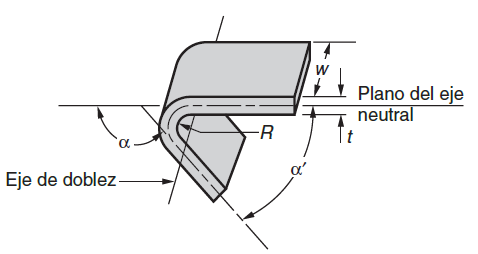
\includegraphics[scale=0.9]{src/ch2/doblado_lamina.png}
\captionof{figure}{Doblado de lámina}
\label{fig:doblado_lamina}
\end{center}

Las operaciones de doblado se realizan usando como herramientas diversos componentes 
que normalmente son conocidos como \textit{formadores}. Los métodos de doblado más 
comunes son el doblado en V, el doblado en U y el doblado de bordes.\\

En el doblado en V la lámina metálica se dobla entre el punzón o formador y una matriz 
en forma de V, como se muestra en la figura \ref{fig:doblado_v}. Los ángulos de doblado 
pueden incluir una variedad de rangos.

\begin{center}
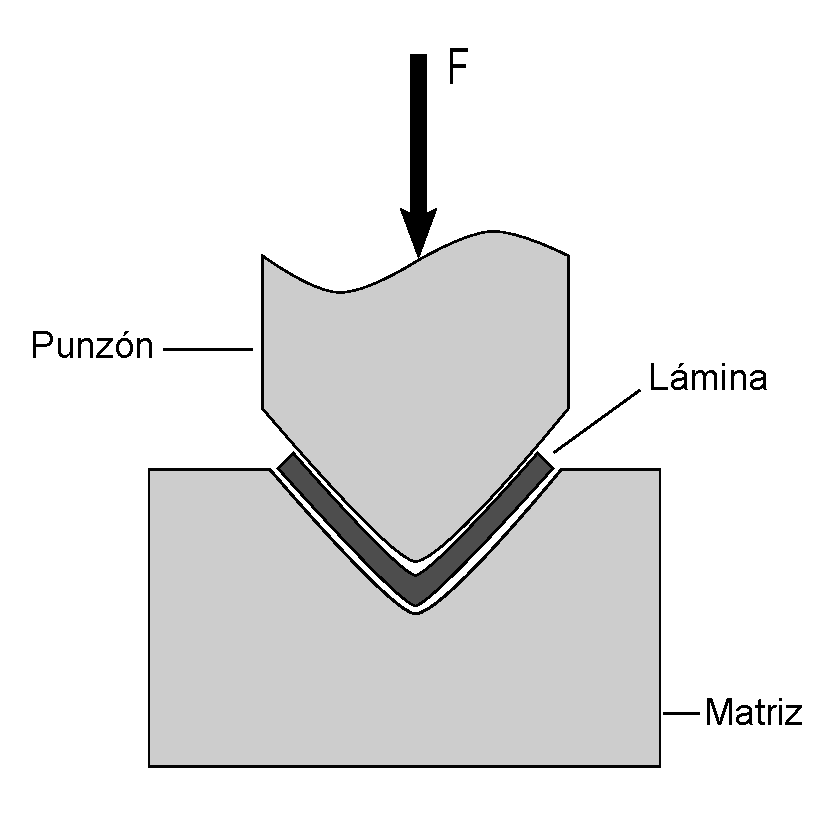
\includegraphics[scale=0.4]{src/ch2/doblado_v}
\captionof{figure}{Doblado en V}
\label{fig:doblado_v}
\end{center}

El doblado en U es muy similar al anterior, con la diferencia que el radio del doblado 
suele ser más amplio, como se muestra en la figura \ref{fig:doblado_u}.

\begin{center}
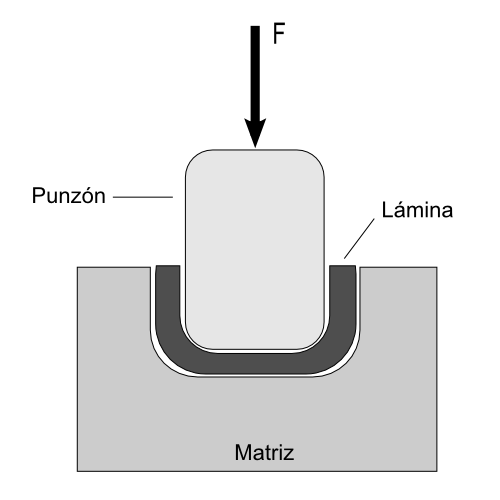
\includegraphics[scale=0.4]{src/ch2/doblado_u}
\captionof{figure}{Doblado en U}
\label{fig:doblado_u}
\end{center}

El doblado de bordes involucra una carga voladiza sobre la lámina de metal. Se utiliza 
un \textit{pisador} que aplica una fuerza de sujeción $F_p$, para sostener la placa de 
metal en una posición adecuada para llevar a cabo el doblado, mientras el punzón 
se desliza en la parte del voladizo para forzar el doblado de la pieza sobre el borde 
de la matriz (ver figura \ref{fig:doblado_bordes}. Normalmente este tipo de doblado 
se limita a ángulos de 90° o menores.

\begin{center}
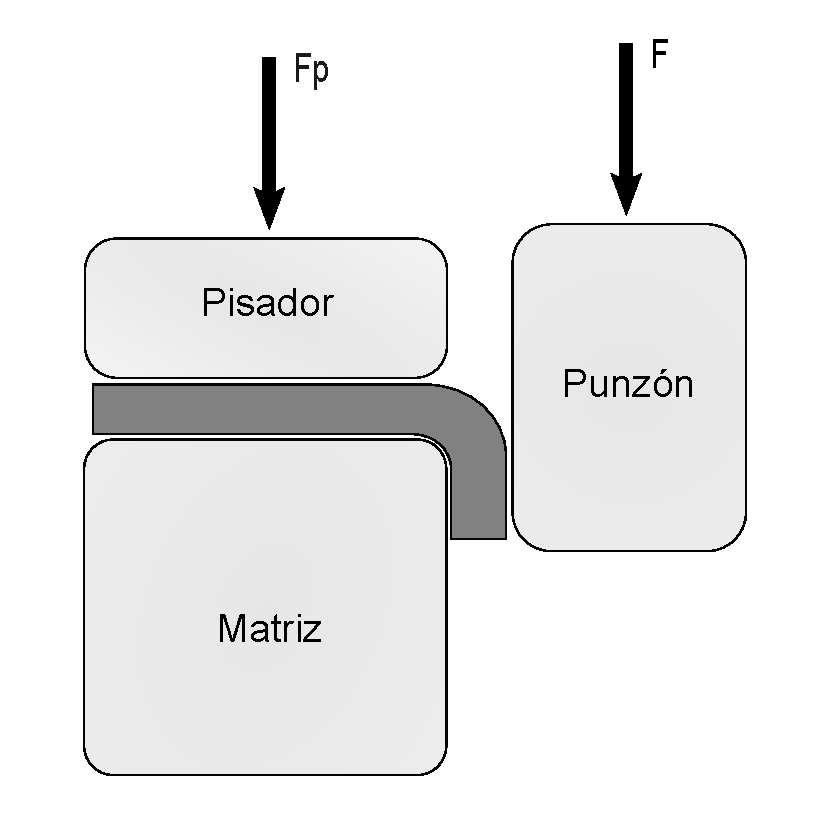
\includegraphics[scale=0.4]{src/ch2/doblado_bordes}
\captionof{figure}{Doblado de bordes}
\label{fig:doblado_bordes}
\end{center}


\subsubsection{Tolerancia de doblado}

En el proceso de doblado es importante tomar en cuenta algunas características relativas a la 
pieza de trabajo. Tomando como referencia la figura \ref{fig:doblado_lamina}, una hoja metálica 
de espesor $t$ se dobla a través de un ángulo llamado ángulo de doblado $\alpha$. El  resultado 
es una pieza doblada con un ángulo incluido $\alpha'$, tal que $\alpha + \alpha' = 180°$. 
El radio de doblado $R$ se especifica normalmente en la parte interna de la pieza, en lugar de 
sobre el eje neutral, y se determina por el radio de la herramienta utilizada para ejecutar 
la operación. El doblado se hace sobre el ancho de la pieza de trabajo $w$. ~\cite{groover2007}\\

Si el radio de doblado es pequeño respecto al espesor del material el metal tiende a estirarse 
durante el doblado. Es importante poder estimar la magnitud del estirado que ocurre, de manera 
que la longitud de la pieza final pueda coincidir con la dimensión especificada. El problema 
es determinar la longitud del eje neutral antes del doblado, para tomar en cuenta el estirado 
de la sección doblada final. Esta longitud se llama \textit{tolerancia de doblado} y se puede 
estimar como sigue: ~\cite{groover2007}

\begin{equation}
A_b = 2\pi \frac{\alpha}{360} \left( R + K_{ba} t \right)
\end{equation}

Donde $A_b$ es la tolerancia de doblado en $mm$, $\alpha$ el ángulo de doblado en grados, 
$R$ el radio de doblado, $t$ el espesor del material y $K_{ba}$ es un factor para estimar 
el estirado. Los siguientes valores de diseño se recomiendan para $K_{ba}$: ~\cite{groover2007}

$$
\left\{
\begin{matrix}
K_{ba} = 0.33 & Si \,\,\, R<2t \\
K_{ba} = 0.5 & Si \,\,\, R>2t \\
\end{matrix} \right.
$$

Estos valores de $K_{ba}$ predicen que el estiramiento ocurre solamente si el radio de doblado 
es más pequeño en relación con el espesor de la lámina.

\subsubsection{Fuerza de doblado}

La fuerza requerida para llevar a cabo un proceso de doblado depende de la configuración del 
herramental, así como de las propiedades mecánicas y geométricas de la pieza de trabajo. 
Con la ecuación \ref{eq:fuerza_doblado} se puede estimar la fuerza máxima de doblado.

\begin{equation}\label{eq:fuerza_doblado}
F = \frac{K S_{t} w t^2}{D}
\end{equation}

Donde $F$ es la fuerza de doblado, $S_t$ la resistencia a la tensión del material, $w$ y $t$ el 
ancho y espesor de la pieza de trabajo, respectivamente, $D$ es la longitud de la parte abierta 
de la matriz, tal como se esquematiza en la figura \ref{fig:fuerza_doblado}. $K$ es una constante 
cuyo valor depende del tipo de doblado, normalmente 1.33 para doblado en V y 0.33 para doblado 
de bordes. ~\cite{groover2007}

\begin{center}
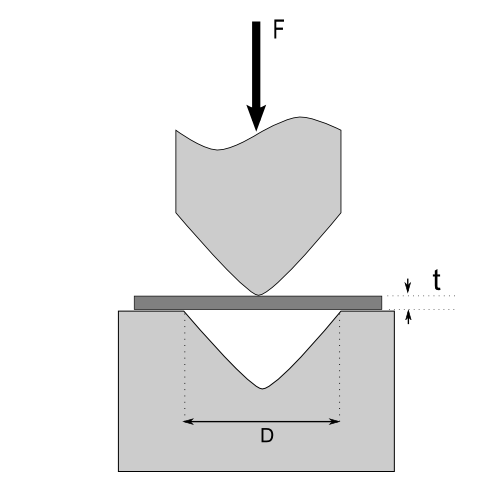
\includegraphics[scale=0.425]{src/ch2/fuerza_doblado}
\captionof{figure}{Esquema de la fuerza de doblado}
\label{fig:fuerza_doblado}
\end{center}


\subsubsection{Recuperación elástica}

Cuando se diseña un troquel, es necesario considerar la recuperación elástica o \textit{springback} 
que ocurre después de la descarga, debido a que el material tiende a recuperar su forma 
inicial e implica que el ángulo de doblado en el herramental $\alpha_i$ no corresponda exactamente con el 
ángulo deseado $\alpha_f$. La recuperación elástica ocurre en todos los tipos de formado 
que implican un tipo de doblado.\\

\begin{center}
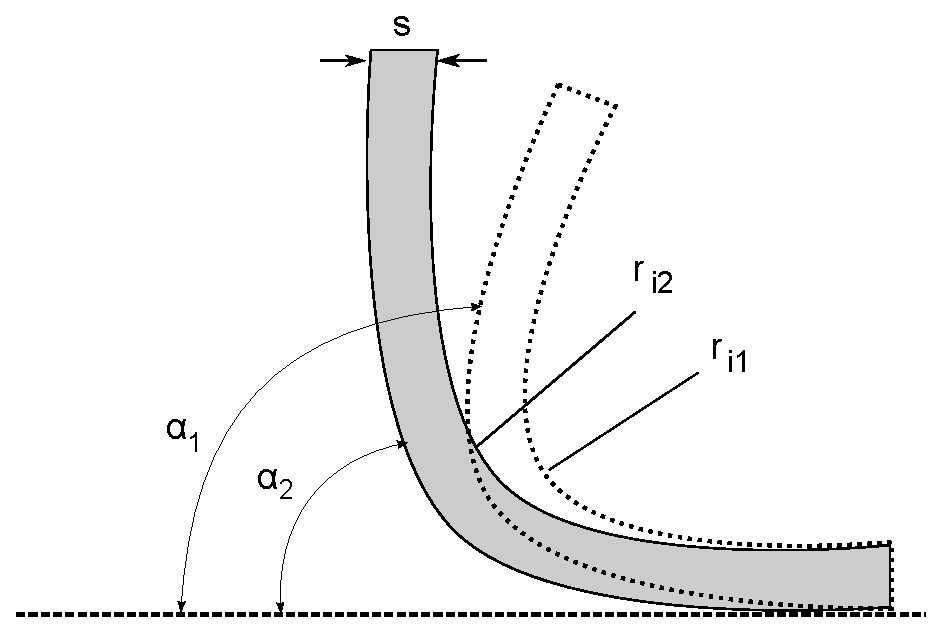
\includegraphics[scale=0.4]{src/ch2/springback}
\captionof{figure}{Recuperación elástica de una pieza metálica sometida a doblez}
\label{fig:springback}
\end{center}

La relación dada entre los ángulos $\alpha_i$ y $\alpha_f$ se conoce como factor de \textit{springback} $k_R$, 
y depende de las características del material y la relación entre el radio de doblez y el espesor de la 
pieza de trabajo. La relación se puede expresar como sigue: ~\cite{schuler1998}

\begin{equation}\label{eq:factor_springback}
k_R = \frac{\alpha_f}{\alpha_i} = \frac{r_{i} + 0.5 s}{r_{f} + 0.5 s}
\end{equation}

Donde, usando como referencia gráfica la figura \ref{fig:springback}, $\alpha_i$ es el ángulo por el 
herramental, $\alpha_f$ el ángulo deseado en la pieza de trabajo (o después del springback), 
$s$ es el espesor de la pieza de trabajo, $r_{i}$ el radio interno en el herramental y $r_{f}$ el 
radio interno en la pieza de trabajo.\\

Luego, el ángulo necesario en el troquel o matriz viene dado por:

\begin{equation}
\alpha_i = \frac{\alpha_f}{k_R}
\end{equation}

El radio interior requerido en el troquel puede ser calculado como:

\begin{equation}
r_{i} = \frac{r_{f}}{1+\frac{r_{f} \cdot S_t}{s \cdot E}}
\end{equation}

Donde $S_t$ es la resistencia a la tensión del material y $E$ el módulo elástico correspondiente.\\

La ecuación \ref{eq:factor_springback} permite calcular la recuperación elástica a si se conoce 
previamente ambos radios internos (antes y después de la descarga). Pero es posible 
predecir la relación $r_i/r_f$ mediante la siguiente ecuación: ~\cite{kalpakjian2008}

\begin{equation}
\frac{r_i}{r_f} = 4 \left( C r_i\right)^3 - 3 \left( C r_i \right) + 1
\end{equation}

Donde $C$ es una constante dada por:

\begin{equation}
C = \frac{S_y}{Es}
\end{equation}

Siendo $S_y$ la esfuerzo de fluencia del material. Esta ecuación nos permite observar 
que la recuperación elástica aumenta cuando lo hacen la relación $r/s$ y el 
esfuerzo de fluencia $S_y$, así como al disminuir el módulo elástico.


\subsection{Herramentales (troqueles)}

Los herramentales utilizados en los procesos de formado (comúnmente llamados troqueles) son 
construidos teniendo en cuenta algunos aspectos elementales, a saber ~\cite{marin2009}:

\begin{enumerate}
\item Trabajo a realizar 
\item Características de la prensa
\item Material a troquelar
\item Número de piezas a producir
\end{enumerate}

\subsubsection{Tipos de troqueles}

A medida que aumentan los requerimientos del trabajo, la capacidad de las prensas, las exigencias 
de los materiales y la necesidad de producir más y mejor, también se conciben los diseños de 
troqueles con mayor complejidad y desarrollo. En ese sentido, los troqueles se pueden clasificar 
en simples, compuestos y progresivos.\\

\textbf{Simples}: estos troqueles permiten realizar solamente una operación por cada golpe o 
ciclo de la prensa, lo cual implica una bajo volumen de producción y productividad, y 
siendo normalmente necesario el uso de más de un herramental para terminar el producto.\\

\textbf{Compuestos}: permiten aprovechar la fuerza ejercida por la prensa realizando dos 
o más operaciones en cada golpe, agilizando el proceso y elevando en cierto punto 
la productividad.\\

\textbf{Progresivos}: son troqueles complejos y de gran desarrollo. Constan de una 
cantidad considerable de etapas, en cada uno de ellos se modifica la lámina con una secuencia 
establecida durante el diseño y acorde a los requerimientos del producto, de tal manera 
que al final se obtiene una o varias piezas terminadas. Naturalmente son altamente productivos, 
aunque su mantenimiento y operación es más compleja que en los casos anteriores.

\subsubsection{Componentes de un troquel}

Los componentes de un troquel varían dependiendo del tipo, pero típicamente hay elementos 
que se encuentran en casi todos los troqueles y que cumplen con funciones específicas 
en el proceso de formado.\\

\textbf{Base superior}. Contiene en su interior todas las placas y elementos que sostienen 
los punzones del troquel, está anclada a la prensa. Algunos elementos alojados en 
la parte superior son: placa porta-punzones, punzones, sufrideras, postes, pisadores, resortes, 
entre otros elementos adicionales.\\


\begin{center}
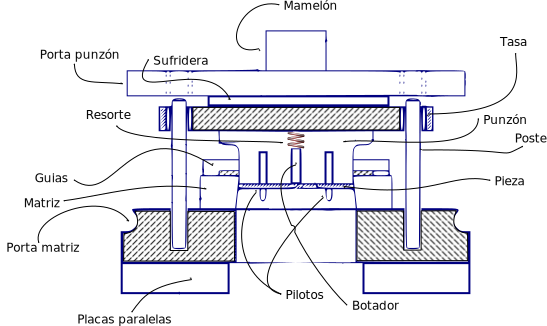
\includegraphics[scale=0.3]{src/ch2/componentes_troquel.png}
\captionof{figure}{Componentes de un troquel. \textit{Fuente:} ~\cite{wikiTroquel2008}}
\label{fig:componentes_troquel}
\end{center}


\textbf{Base inferior}. Es el elemento sobre el cual van montados todos los componentes 
que hacen la parte de la matriz, y a su vez, está fuertemente sujeta en la bancada 
de la prensa durante la fase de trabajo. Algunos de los elementos contenidos en 
la base inferior son: placa  porta-matrices, guías, sufrideras, topes de avance, entre 
otros.\\

\textbf{Sufrideras}. La función básica de las placas superior e inferior de choque o sufrideras 
consiste en absorber sobre su superficie los sucesivos golpes de los elementos en el troquel. 
Estos impactos se producen cada vez que los punzones transforman la lámina con la matriz. Cuando 
el punzón impacta contra el material, la resistencia que opone este es transmitida a la 
superficie de las sufrideras sobre las que se apoyan las placas porta matriz y porta punzones. 
Estas placas están construidas en materiales ya templados y que conservan su tenacidad y cohesión, 
uno muy empleado es el acero SAE/AISI 1045.\\

\textbf{Porta punzones}. La finalidad de la placa porta punzones es la de alojar y fijar en 
su interior todos los punzones que lleve la matriz. Estos punzones pueden ser de cualquier 
tipo o tamaño pero han de tener una sola carcterística en común: deben estar firmemente 
sujetos y guiados en el interior de dicha placa impidiendo que puedan moverse o desprenderse.\\

\textbf{Porta matriz}. La placa porta matrices aloja y posiciona en su interior todos 
los elementos de pequeñas dimensiones que lleve la propia matriz, de esta manera dichos componentes 
quedarán ajustados en su interior.\\

\textbf{Placa pisadora}. Durante el movimiento descendente del troquel, la placa pisadora presiona 
la lámina dejándola inmovilizada antes de que los punzones lleguen a tocarla y mientras penetran 
el material y lo transforman. Una vez cortada la lámina, la función de la placa es mantener la 
pieza bien sujeta hasta que los punzones hayan salido de ella, de lo contrario, los punzones 
la arrastrarían hacia arriba sujeta a ellos, con el riesgo de fractura.\\

\textbf{Punzones}. Los punzones tienen por objeto realizar las máximas transformaciones en la lámina 
a fin de obtener piezas con una calidad acorde a las medidas requeridas, hay tanto tipos de estos 
como variantes del troquelado.\\

\textbf{Matrices}. Las matrices son los elementos complementarios a los punzones, tienen la forma 
negativa de estos.

% ====================================================================================================
% ======================================== Teoría de plasticidad =====================================
% ====================================================================================================

\section{Teoría de plasticidad}

La teoría de plasticidad estudia la fluencia de materiales bajo estados de esfuerzos complejos. Permite 
conocer si un material cederá bajo ciertas condiciones de esfuerzo y determinar el cambio en la forma o 
geometría en caso de que la fluencia ocurra. También permite usar datos de ensayos de tensión para predecir 
el endurecimiento por carga durante la deformación bajo complejos estados de esfuerzo. Estas relaciones 
son parte fundamental de los códigos de computadora utilizados para predecir la capacidad de una estructura 
para absorber impactos, así como en procesos de formado o estampado que involucran la deformación plástica de 
placas metálicas. ~\cite{hosford2005}

\subsection{Esfuerzos, deformaciones y tasa de deformación}

Las cantidades elementales que pueden ser usadas para describir los mecanismos de deformación 
cuando un sólido se deforma de una configuración a otra bajo la influencia de cargas externas 
son los esfuerzos, deformaciones y la tasa de deformación. ~\cite{kobayashi1989} \\

Considere el ensayo de tensión uniaxial de un especimen cilíndrico cuya longitud inicial 
es $l_0$ y un área transversal $A_0$. El especimen se reduce en la dirección axial 
por acción de la fuerza $P$ a la longitud $l$ y sección transversal $A$ en el tiempo 
$t$, como se observa en la figura \ref{fig:tensile_test}. El comportamiento del material 
se caracteriza como una curva carga-desplazamiento, y se convierte a una de 
esfuerzo-deformación como se muestra en la figura \ref{fig:tensile_test}. La deformación 
se asume homogénea hasta que se presentan grietas. ~\cite{kobayashi1989} \\

\begin{center}
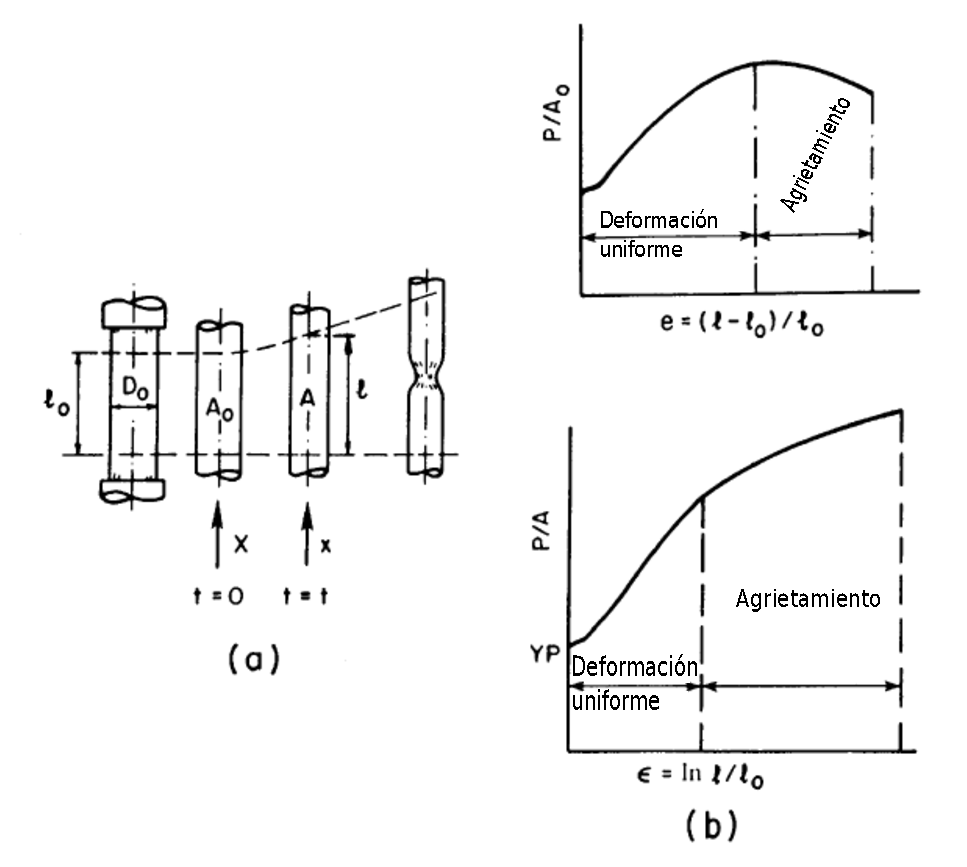
\includegraphics[scale=0.8]{src/ch2/tensile_test.png}
\captionof{figure}{Ensayo de tensión uniaxial a) Especimen b) Curva esfuerzo-deformación}
\label{fig:tensile_test}
\end{center}

Hay dos formas de describir la deformación de un medio continuo: la lagrangiana y la euleriana. 
La descripción lagrangiana utiliza las coordenadas $X_i$ de una partícula típica en el estado 
de referencia (o sin deformar) como las variables independientes, mientras en el caso 
de la descripción euleriana la descripción de las variables independientes son las coordenadas 
$x_i$ de un punto material en el estado deformado. Cuando la deformación es infinitesimal, los 
productos de las derivadas de desplazamiento pueden ser \textit{despreciados}, y entonces no 
se hace una distinción entre ambos enfoques. ~\cite{kobayashi1989} \\

En la teoría de deformación infinitesimal, las esfuerzos y las tasas de deformación son expresadas 
con respecto a un sistema fijo de coordenadas en la configuración actual del material en 
un tiempo determinado. Para el caso de tensión uniaxial se tiene: ~\cite{kobayashi1989}

\begin{align}
\sigma = \frac{P}{A} \\
\dot{\varepsilon} = \frac{\dot{l}}{l} \\
d\varepsilon = \frac{dl}{l}
\end{align}

Los esfuerzos definidos en la ecuación anterior son llamados esfuerzos verdaderos o 
esfuerzo de Cauchy. La cantidad total de deformación se obtiene integrando las deformaciones 
infinitesimales:

\begin{equation}
\varepsilon = \int_{l_0}^{l} d\varepsilon = \ln{\frac{l}{l_0}}
\end{equation}

y es llamada deformación logarítmica o natural.\\

En la descripción lagrangiana de la deformación finita, la medida de los esfuerzos, 
deformaciones y tasa de deformación son expresadas como sigue. Sea la posición 
de una partícula en su configuración deformada en el tiempo $t$ la designada por: 

\begin{equation}
x = \chi(X,t)
\end{equation}

donde $X$ es una posición de referencia de una partícula y $t$ el tiempo. En 
tensión uniaxial sea $X$ una posición a lo largo del eje longitudinal del 
especimen de la figura \ref{fig:tensile_test}, entonces:

\begin{equation}
x = X + \left( \frac{l-l_0}{l_0} \right) X
\end{equation}

La elongación se define como el gradiente del desplazamiento relativo a la posición 
de referencia y se expresa como:

\begin{equation} \label{eq:disp_grad}
\frac{\partial (x-X)}{\partial X} = \frac{l-l_0}{l_0} = e
\end{equation}

Esto es el esfuerzo ingenieril o de ingeniería. \\

La componente de deformación lagrangiana $E_{11}$ está definida por:

\begin{equation} \label{eq:lagra_strain}
E_{11} = \frac{1}{2} \left( \frac{\partial x}{\partial X} \frac{\partial x}{\partial X} - 1 \right) = 
\frac{1}{2} \left[ (1+e)^2 - 1 \right] = e + \frac{1}{2} e^2
\end{equation}

% [REFERENCIA]: Revisar referencia para interpretación geométrica 

Los componentes de la tasa de deformación son las derivadas del tiempo de las componentes 
de deformación dadas por las ecuaciones \ref{eq:disp_grad} y \ref{eq:lagra_strain}, y son:

\begin{equation}
\dot{e} = \frac{\dot{l}}{l_0}
\end{equation}

y 

\begin{equation}
\dot{E_{11}} = \frac{\partial x}{\partial X} \frac{\partial \dot{x}}{\partial X} = 
(1+e)\dot{e}
\end{equation}

siendo:

\begin{equation}
\dot{x} = \frac{\partial \chi}{\partial t} \Big\rvert_{X = const.}
\end{equation}

Para el análisis de procesos de formado, la formulación de flujo está basada la teoría 
de deformación infinitesimal, mientras la formulación sólida considera deformaciones 
finitas. \\

El tensor de la tasa de deformacion $[\dot{\varepsilon_{ij}}]$, donde $i,j = x,y,z$ es simétrico 
y los componentes del tensor están definidos por: 

\begin{eqnarray} \label{eq:strain_rate_tensor}
\dot{\varepsilon_x} = \frac{\partial u_x}{\partial x} \,\,\,\,\, ;
\dot{\varepsilon_x} = \frac{\partial u_x}{\partial x}  \,\,\,\,\, ;
\dot{\varepsilon_x} = \frac{\partial u_x}{\partial x} \\
\dot{\varepsilon_{xy}} = \frac{1}{2} \left( \frac{\partial u_x}{\partial y} + \frac{\partial u_y}{\partial x} \right) = \frac{\dot{\gamma_{xy}}}{2} \\
\dot{\varepsilon_{yz}} = \frac{1}{2} \left( \frac{\partial u_y}{\partial z} + \frac{\partial u_z}{\partial y} \right) = \frac{\dot{\gamma_{yz}}}{2} \\
\dot{\varepsilon_{zx}} = \frac{1}{2} \left( \frac{\partial u_z}{\partial x} + \frac{\partial u_x}{\partial z} \right) = \frac{\dot{\gamma_{zx}}}{2}
\end{eqnarray}

Donde $u_i$ son componentes de velocidad y $\gamma_{ij}$ son componentes de la tasa 
deformación por cortante ingenieril. Utilizando notación de subíndices, la ecuación 
\ref{eq:strain_rate_tensor} puede ser reescrita como:

\begin{equation}
\dot{\varepsilon_{ij}} = \frac{1}{2} \left( u_{i,j} + u_{j,i} \right)
\end{equation}

Donde las comas denotan la derivación respecto a las coordenadas que siguen.\\

El tensor de esfuerzos de Cauchy $[\sigma_{ij}]$, donde $i,j = 1,2,3$ o $x,y,z$, es 
también simétrico y es representado por los nueve componentes como sigue:

\begin{equation}
[\sigma_{ij}] = 
\begin{bmatrix}
\sigma_{11} & \sigma_{21} & \sigma_{31} \\
\sigma_{12} & \sigma_{22} & \sigma_{32} \\
\sigma_{13} & \sigma_{23} & \sigma_{33} 
\end{bmatrix}
=
\begin{bmatrix}
\sigma_x & \tau_{yx} & \tau_{zx} \\
\tau_{xy} & \sigma_y & \tau_{zy} \\
\tau_{xz} & \tau_{yz} & \sigma_z 
\end{bmatrix}
\end{equation}

El esfuerzo puede también especificarse por sus tres componentes principales, o por 
los tres invariantes. Los esfuerzos principales ($\sigma_1, \sigma_2, \sigma_3$), son 
ráices de la ecuación cúbica:

\begin{equation}
\sigma^3 - I_1 \sigma^2 - I_2 \sigma - I_3 = 0
\end{equation}

Donde $I_1$, $I_2$ e $I_3$ son cantidades independientes de la dirección de los ejes 
seleccionados y son llamados los tres invariantes del tensor de esfuerzos $\sigma_{ij}$, y están definidos 
por las relaciones:

\begin{align}
I_1 = \sigma_x + \sigma_y + \sigma_z = \sigma_1 + \sigma_2 + \sigma_3 \\
I_2 = -\left( \sigma_x \sigma_y + \sigma_y \sigma_z + \sigma_z \sigma_x \right) + \tau_{xy}^2 + 
\tau_{yz}^2 + \tau_{zx}^2 = -(\sigma_1 \sigma_2 + \sigma_2 \sigma_3 + \sigma_3 \sigma_1) \\
I_3 = \sigma_x \sigma_y \sigma_z + 2 \tau_{xy} \tau_{yz} \tau_{zx} - \sigma_x \tau_{yz}^2 - \sigma_y \tau_{zx}^2 - 
\sigma_z \tau_{xy}^2 = \sigma_1 \sigma_2 \sigma_3
\end{align}

El primer y segundo invariantes tienen importancia física en la teoría de plasticidad.\\




\subsection{Criterio de fluencia}

Un criterio de fluencia es una expresión matemática propuesta del estado de esfuerzo que causará 
la fluencia. La forma más general es: ~\cite{hosford2005}

\begin{equation}
f(\sigma_x,\sigma_y, \sigma_z, \tau_{yz}, \tau_{zx}, \tau_{xy} ) = C 
\end{equation}

Donde C es una constante del material. Para materiales isotrópicos esto puede ser expresado en 
términos de los esfuerzos principales como: ~\cite{hosford2005}

\begin{equation}
f(\sigma_1,\sigma_2,\sigma_3 )=C
\end{equation}

Para la mayoría de los metales dúctiles isotrópicos comúnmente se hacen las siguientes 
consideraciones: ~\cite{hosford2007}


\begin{itemize}
\item El esfuerzo de fluencia en tensión y compresión es el mismo.
\item El volumen permanece constante durante la deformación plástica
\item La magnitud del esfuerzo normal promedio, no afecta la fluencia.
\end{itemize}

\begin{equation}
\sigma_m=\frac{\sigma_1+\sigma_2+\sigma_3}{3}
\end{equation}

La consideración que la fluencia es independiente de $\sigma_m$ es razonable porque la deformación 
usualmente ocurre por deslizamiento o mecanismos de corte. Por lo tanto los criterios de fluencia 
para materiales isotrópicos tienen la forma: ~\cite{hosford2007}

\begin{equation}
f[(\sigma_2-\sigma_3 ),(\sigma_3-\sigma_1 ),(\sigma_1-\sigma_2 )] = C
\end{equation}

Esto es equivalente a considerar que la fluencia depende sólo del tamaño del círculo de Mohr, 
y no de su posición, la figura \ref{fig:circulos_mohr} muestra esto. Si el estado de esfuerzos 
$\sigma_1$, $\sigma_2$, $\sigma_3$, causará la fluencia, otro estado de efuerzos 
$\sigma_1' = \sigma_1 - \sigma_m $, $\sigma_2' = \sigma_2 - \sigma_m $, $\sigma_3' = \sigma_3 - \sigma_m $, 
que difiere sólo por $\sigma_m$, también causará la fluencia. Estos esfuerzos $\sigma_1'$, $\sigma_2'$, 
$\sigma_3'$ se conocen como esfuerzos desviatorios. ~\cite{hosford2007}

\begin{center}
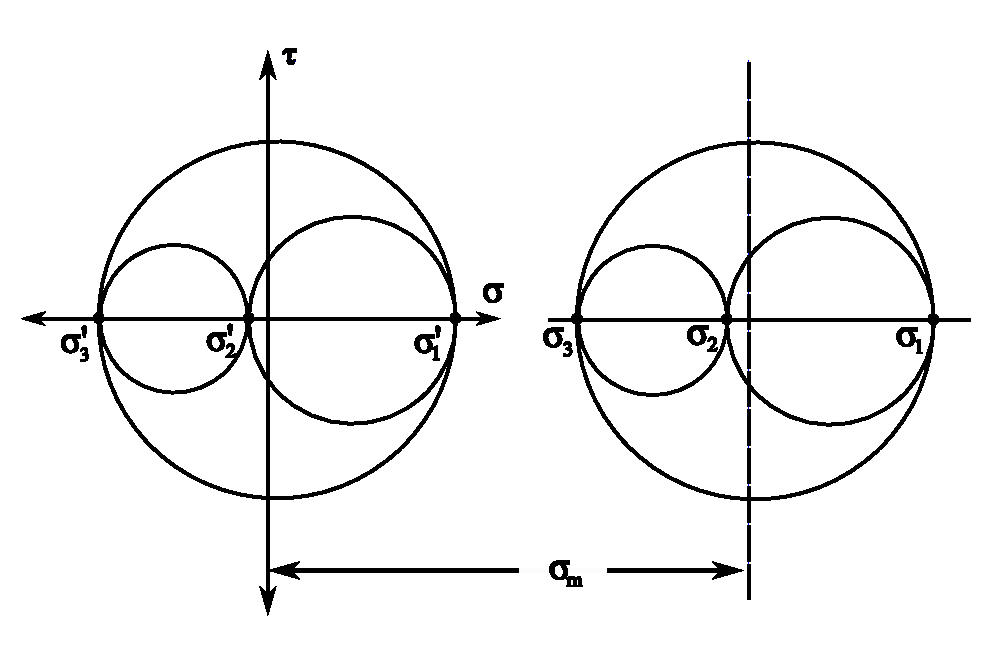
\includegraphics[scale=0.75]{src/ch2/circulos_mohr_svg}
\captionof{figure}{Círculos de Mohr para dos estados de esfuerzos que difieren por un esfuerzo hidrostático, $\sigma_m$ y que son equivalentes en términos de la fluencia}
\label{fig:circulos_mohr}
\end{center}



% =========================================== Criterio de tresca =============================================
\subsubsection{Criterio de Tresca}

El criterio más simple es uno de los primero propuestos por Tresca. Afirma que la cedencia 
ocurrirá cuando el máximo esfuerzo cortante alcance un valor crítico. El máximo esfuerzo 
cortante viene dado por:

\begin{equation}
\tau_{max} = \frac{\sigma_{max}-\sigma_{min}}{2}
\end{equation}

entonces, el criterio de Tresca puede expresarse como:

\begin{equation}
\sigma_{max} - \sigma_{min} = C
\end{equation}

Si se mantiene la convención de que $ \sigma_1 \me \sigma_2 \me \sigma_3 $, puede reescribirse lo anterior como:

\begin{equation}\label{eq:ec1}
\sigma_1 - \sigma_3 = C
\end{equation}

La constante C puede ser encontrada mediante un ensayo de tensión uniaxial. En un ensayo de tensión, 
$\sigma_2 = \sigma_3 = 0$ y la cedencia $\sigma_1 = Y$, donde $Y$ es el esfuerzo de fluencia. Sustituyendo 
en $C=Y$ en la ecuación \ref{eq:ec1}. Por lo tanto el criterio de Tresca puede ser expresado como:

\begin{equation}\label{eq:ec2}
\sigma_1 - \sigma_3 = Y
\end{equation}

Para cortante puro, $ \sigma_1 = -\sigma_3 = k$, donde $k$ es esfuerzo de fluencia por cortante. Sustituyendo 
$ k = Y/2 $ en la ecuación \ref{eq:ec2}, entonces:

\begin{equation}
\sigma_1 - \sigma_3 = 2k = C
\end{equation}

\subsubsection{Criterio de Von Mises}

El efecto del esfuerzo principal medio puede ser incluido asumiendo que la fluencia depende de la raíz cuadrada 
del promedio de los diámetros de los tres círculos de Mohr. Este es el criterio de Von Mises, el cual puede ser 
expresado como:

\begin{equation} \label{eq:ec3}
\left( \frac{ (\sigma_2-\sigma_3)^2 + (\sigma_3-\sigma_1 )^2 + (\sigma_1-\sigma_2)}{3} \right) ^{1/2} = C
\end{equation}

Como cada término está elevado al cuadrado, la convención $\sigma_1 \geq \sigma_2 \geq \sigma_3$ no es necesaria. 
La constante del material, $C$, puede ser evaluada mediante un ensayo de tensión uniaxial. En la fluencia, 
$\sigma_1 = Y$ y $\sigma_2 = \sigma_3 = 0$. Sustituyendo, $[0^2 + (-Y)^2 + Y^2]/3 = C^2$, o 
$C = (2/3)^{1/3} Y $, entonces, la ecuación usualmente se escribe como:

\begin{equation}\label{eq:ec4}
(\sigma_2-\sigma_3)^2 + (\sigma_3-\sigma_1 )^2 + (\sigma_1-\sigma_2 )^2 = 2Y^2
\end{equation}

Para cortante puro, $\sigma_1 = -\sigma_3 = k$ y $\sigma_2=0$. Sustituyendo en la ecuación \ref{eq:ec4}, 
$ (-k)^2 + [ (-k)-k ]^2 + k^2 = 2Y^2 $, entonces:

\begin{equation}\label{eq:ec5}
k = Y / \sqrt{3}
\end{equation}

La ecuación \ref{eq:ec5} puede ser simplificada si uno de los esfuerzos principales es cero (condición de esfuerzo plano). 
Sustituyendo $\sigma_3 = 0$, $\sigma_1^2 + \sigma_2^2 - \sigma_1 \sigma_2 = Y^2$, el cual es una elipse. Con la 
consiguiente sustitución de $\alpha = \sigma_2/\sigma_1$,

\begin{equation}
\sigma_1 = \frac{y}{(1-\alpha+\alpha^2)^{1/2}}
\end{equation}

El criterio de fluencia de Von Mises puede ser expresado en términos de los esfuerzos que no son principales. 
En este caso es necesario incluir los términos de cortante:

\begin{equation}
(\sigma_y - \sigma_z)^2 + (\sigma_z - \sigma_x)^2 + (\sigma_x - \sigma_y)^2 + 6 (\tau_{yz}^2 + \tau_{zx}^2 + \tau_{xy}^2) = 2Y^2
\end{equation}

donde x, y, z, son esfuerzos en esas direcciones, que no necesariamente son las direcciones principales.


\subsection{Reglas de flujo}

Las deformaciones resultantes en la región elástica son descritas por la ley de Hooke. 
Hay una relación similar para las deformaciones plásticas, llamadas reglas de flujo. 
En el caso más general, la forma de una regla de flujo puede escribirse como: ~\cite{hosford2007}

\begin{equation}
d\varepsilon_{ij} = d\lambda (\partial f / \partial \sigma_{ij})
\end{equation}

Donde $f$ es la función de $\sigma_{ij}$ que describe la fluencia. Esto está relacionado 
con el por qué ha sido llamado el \textit{potencial plástico}. Para el criterio de 
Von Mises, la diferenciación resulta en: ~\cite{hosford2007}

\begin{align}
d\varepsilon_1 = d\lambda \left[ \sigma_1 - (1/2) (\sigma_2 + \sigma_3) \right] \\
d\varepsilon_2 = d\lambda \left[ \sigma_2 - (1/2) (\sigma_3 + \sigma_1) \right] \\
d\varepsilon_3 = d\lambda \left[ \sigma_3 - (1/2) (\sigma_1 + \sigma_2) \right]
\end{align}

En estas expresiones $d\lambda = d \overline{\varepsilon} / \overline{\sigma} $, el cual varía 
con la posición en la curva $ \overline{\sigma} - \overline{\varepsilon} $. Sin embargo, la 
relación de las deformaciones plásticas permanece constante: ~\cite{hosford2007} \\

% \begin{equation}
% d\varepsilon_1 : d\varepsilon_2 : d\varepsilon_3  = 
% \left\[ \sigma_1 - (1/2) (\sigma_2 + \sigma_3) \right\] :
% \left\[ \sigma_2 - (1/2) (\sigma_3 + \sigma_1) \right\] :
% \left\[ \sigma_3 - (1/2) (\sigma_1 + \sigma_2) \right\]
% \end{equation}

Para el criterio de Tresca, $f = \sigma_1 - \sigma_3$, entonces las reglas de flujo son simples:
~\cite{hosford2007}

\begin{align*}
d\varepsilon_1 = dl \\
d\varepsilon_2 = 0 \\
d\varepsilon_3 = -dl
\end{align*}


\subsection{Endurecimiento por deformación}

En el caso unidimensional, un especimen se deformará hasta la fluencia y entonces generalmente 
endurece, como se muestra en la figura \ref{fig:strain_stress_hardening}. En el caso de 
plasticidad perfecta, una vez que el esfuerzo alcanza el punto de fluencia $A$, le sigue una 
deformación plástica siempre y cuando el esfuerzo se mantenga en $Y$. Si el esfuerzo se reduce, 
una descarga elástica ocurre. En el caso con efectos de endurecimiento, una vez que la fluencia 
ocurre, el esfuerzo necesita continuar incrementando para producir la deformación plástica. 
Si el esfuerzo se mantiene constante, por ejemplo en $B$, no ocurrirá una deformación plástica, 
además tampoco sucederá una descarga elástica como en el caso idealizado. ~\cite{kelly2012}

\begin{center}
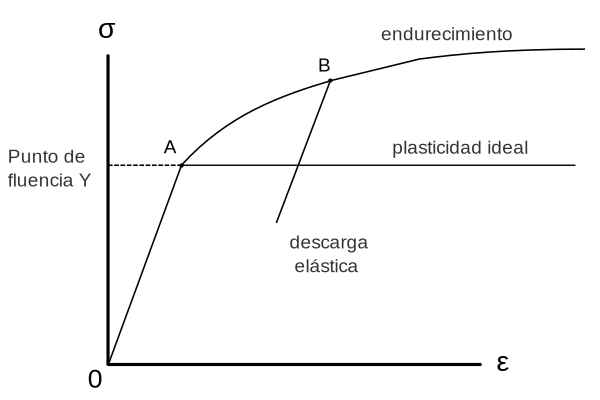
\includegraphics[scale=0.6]{src/ch2/strain_stress_hardening}
\captionof{figure}{Curva esfuerzo-deformación}
\label{fig:strain_stress_hardening}
\end{center}


Estas ideas pueden ser extendidas al caso multiaxial, donde la superficie de fluencia inicial 
tendrá la forma:

\begin{equation}
f_0 (\sigma_{ij}) = 0
\end{equation}

En el caso de plasticidad perfecta, la superficie de fluencia permanece invariable. En el caso 
más general, la superficie de fluencia puede cambiar de tamaño, forma y posición, y puede ser 
descrita por:

\begin{equation}
f(\sigma_{ij}, K_i) = 0
\end{equation}

Donde $K_i$ representa uno o más parámetros de endurecimiento, los cuales cambian durante la 
deformación plástica y determinan la evolución de la superficie de fluencia. Estos pueden 
ser escalares o tensores de orden superior. Al inicio de la fluencia, los parámetros de 
endurecimiento son cero, y $f(\sigma_{ij}, 0) = f_0(\sigma_{ij}) $. \\

La descripción de cómo la superficie de fluencia cambia con la deformación plástica es 
llamada regla de endurecimiento. 

\subsubsection{Endurecimiento isotrópico}

El endurecimiento isotrópico es cuando la superficie de fluencia permance en la misma forma, 
pero se expande cuando el esfuerzo aumenta, tal como se esquematiza en la figura \ref{fig:isotropic_hardening}.

\begin{center}
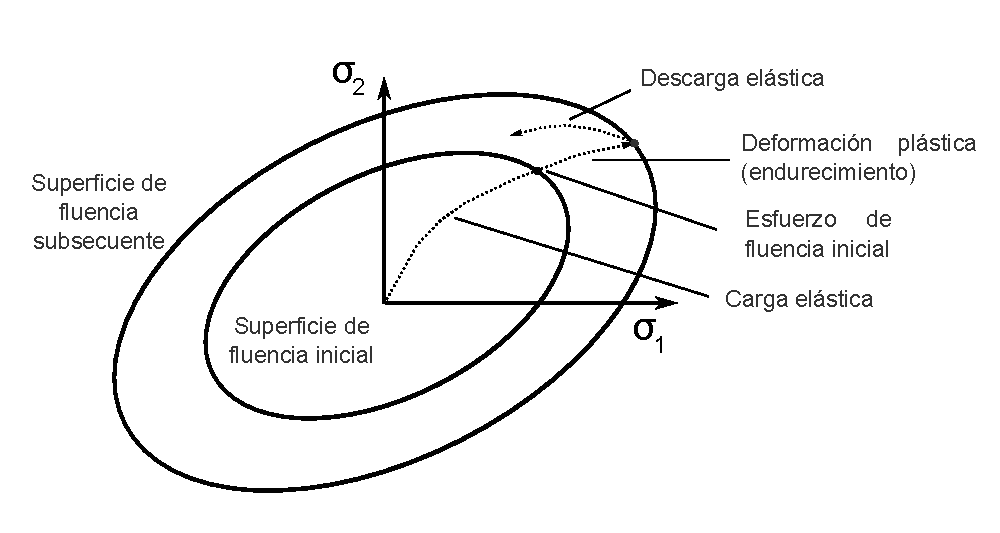
\includegraphics[scale=0.8]{src/ch2/isotropic_hardening}
\captionof{figure}{Endurecimiento isotrópico}
\label{fig:isotropic_hardening}
\end{center}

En particular, la función de fluencia toma la forma:

\begin{equation}
f(\sigma_{ij}, K_i) = f_0 ( \sigma_{ij} ) - K = 0
\end{equation}

La forma de la función de fluencia es especificada por la función de fluencia inicial y su 
tamaño cambia conforme lo hace el parámetro de endurecimiento $K$.


\subsubsection{Endurecimiento cinemático}

El modelo isotrópico implica que, si el esfuerzo de fluencia en tensión y compresión son 
inicialmente iguales, estos permanecen iguales a como la superficie de fluencia se desarrolla 
con la deformación plástica. Con la finalidad de modelar el efecto de Bauschinger y comportamientos 
similares, donde un endurecimiento a tensión dará lugar a un ablandamiento en una compresión 
subsecuente, se puede entonces utilizar la regla de endurecimiento cinemático. En esta 
la superficie de fluencia permanece de la misma forma y tamaño, pero conlleva una traslación simple 
en el espacio de esfuerzos, como se muestra en la figura \ref{fig:kinematic_hardening}


\begin{center}
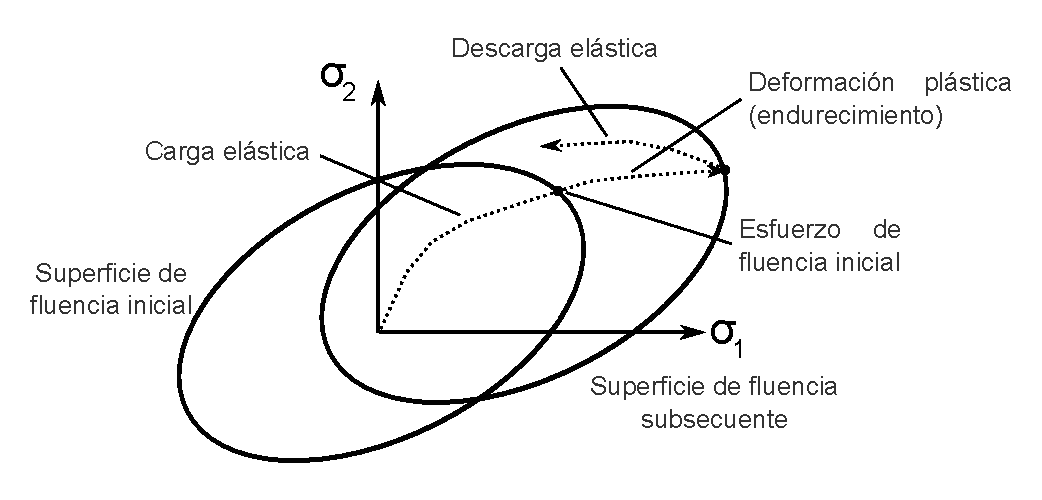
\includegraphics[scale=0.8]{src/ch2/kinematic_hardening}
\captionof{figure}{Endurecimiento cinemático}
\label{fig:kinematic_hardening}
\end{center}

La función de fluencia ahora toma la forma general:

\begin{equation}
f(\sigma_{ij}, K_i) = f_0 (\sigma_{ij} - \alpha_{ij}) = 0
\end{equation}

Aquí el parámetro de endurecimiento es el esfuerzo $\alpha_{ij}$, conocido como \textit{back-stress}; 
la superficie de fluencia se desplaza respecto a los ejes del espacio de esfuerzos por $\alpha_{ij}$, 
como se muestra en la figura \ref{fig:shift_back_stress}

\begin{center}
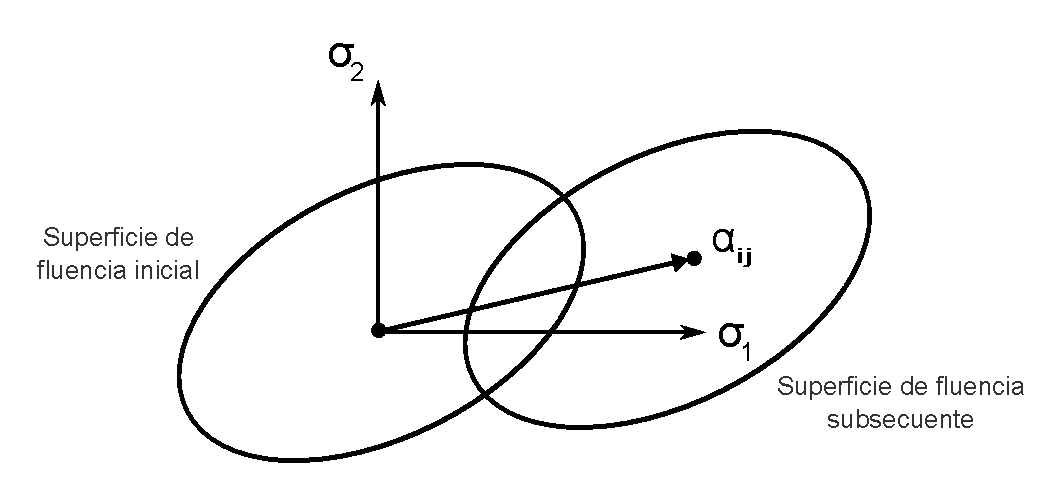
\includegraphics[scale=0.8]{src/ch2/shift_back_stress}
\captionof{figure}{Endurecimiento cinemático: desplazamiento por el \textit{back-stress} }
\label{fig:shift_back_stress}
\end{center}


% ================================================================================================================
% ================================= 	MÉTODO DE LOS ELEMENTOS FINITOS ==========================================
% ================================================================================================================

\section{El método de los elementos finitos}

\subsection{Una introducción al método}

En el método de elementos finitos se considera un cuerpo continuo o sólido, como un ensamble de pequeñas 
subdivisiones llamadas elementos finitos. Estos elementos están interconectados a través de nodos comunes. 
Debido a que la variación real de las variables de campo (desplazamientos, esfuerzos, temperaturas, etc.) 
se desconoce en el continuo, se asume que la variación de estas en el modelo de elemento finito puede ser 
aproximada por una simple función. Estas funciones de aproximación, también llamadas modelos de interpolación, 
son definidas en términos de los valores nodales de las variables de campo.\\

En general, el método de los elementos finitos, consiste en formular un sistema de ecuaciones 
(ecuaciones de equilibrio) para el sistema continuo que ha sido discretizado, donde las incógnitas 
suelen ser los valores nodales de las variables de campo. Luego, se resuelve este sistema de ecuaciones, 
con las consideraciones correspondientes a las condiciones de frontera o valores iniciales que simplifiquen 
el modelo original. La siguiente ecuación muestra, en notación matricial, el sistema de ecuaciones resuelto 
en una formulación de elemento finito.

\begin{equation} \label{eq:fem_simple}
K\,\vec{u} = \vec{P}
\end{equation}

Donde $K$ es la matriz global de rigidez, $\vec{u}$ es el vector de desplazamientos nodales y $\vec{P}$ el 
vector de fuerzas nodales en el sistema.\\

Para problemas lineales, el vector $\vec{u}$ puede ser resuelto de manera sencilla, mediante 
procedimientos básicos del álgebra lineal. Sin embargo, para problemas no lineales, la solución 
tiene que ser obtenida mediante una secuencia de pasos, en el cual cada uno de estos implica la 
modificación de la matriz de rigidez $K$ y/o el vector global de carga $\vec{P}$.\\

En problemas de análisis dinámico, desplazamientos, velocidades, deformaciones, esfuerzos y cargas 
son dependientes del tiempo. Por ello deben incluirse algunos otros términos, por lo que la ecuación 
a resolver viene dada por la expresión siguiente:

\begin{equation}
M\ddot{\vec{u}} + C\dot{\vec{u}} ̇+ K\vec{u} = \bf{P}
\end{equation}

Donde $C\,\dot{u}$ representa las fuerzas viscosas, mismas que deben incluirse cuando el 
sistema esté amortiguado artificialmente y $M$ la matriz de masas.\\

\subsection{Discretización de un modelo continuo}

En un cuerpo discretizado, su deformación viene definida por un número finito de parámetros 
que conforman el vector de desplazamientos $\vec{u}$. Un medio continuo tiene infinitas formas 
posibles de deformarse, independientes unas de otras, ya que cada punto puede desplazarse 
manteniendo fijos cualquier número finito de los puntos restantes, por grande que sea este 
último. Luego, la configuración deformada es una función vectorial $\vec{u}$, que indica cuáles 
son las deformaciones de cualquier punto, y que tiene tres componentes escalares: ~\cite{celigueta2011}

\begin{equation}
\vec{u} = \left\{ 
\begin{matrix}
u(x,y,z) \\
v(x,y,z) \\
w(x,y,z)
\end{matrix}
\right\}
\end{equation}

Esta función es la solución de la ecuación diferencial que gobierna el problema, y si éste 
está bien planteado, cumplirá las condiciones de contorno impuestas, pero en principio no 
puede asegurarse que esta función tenga una expresión analítica manejable, ni siquiera que 
pueda calcularse. Por lo tanto la función $\vec{u}$ no podrá conocerse en general.

Para resolver este problema el método de los elementos finitos recurre a la hipótesis de 
discretización, que se basa en lo siguiente: ~\cite{zienkiewicz2005} \\

\begin{itemize}
\item El continuo se divide por medio de líneas o superficies imaginarias, en un número 
de elementos finitos.
\item Se supone que los elementos están conectados entre sí mediante un número discreto de puntos, 
que llamaremos nodos, situados en sus contornos. Los desplazamientos de estos nodos serán las 
incógnitas fundamentales del problema, tal como ocurre en el análisis simple de estructuras.
\item Se toma un conjunto de funciones que definan de manera única el campo de desplazamientos 
dentro de cada elemento finito en función de los desplazamientos nodales de dicho elemento.
\item Estas funciones de desplazamientos definirán entonces de manera única el estado de 
deformación dentro del elemento en función de los desplazamientos nodales. Estas deformaciones, 
junto con las deformaciones iniciales y las propiedades constitutivas del material, definirán el 
estado de tensiones en todo el elemento y, por consiguiente, también en sus contornos.
\item Se determina un sistema de fuerzas concentradas en los nodos, tal que equilibre las tensiones 
en el contorno y cualesquiera cargas repartidas, resultando así una relación entre fuerzas y 
desplazamientos como la descrita en la ecuación \ref{eq:fem_simple}.
\end{itemize}

Esta hipótesis de discretización es el pilar básico del método de los elementos finitos, 
el cuál es un método discretizante, de parámetros distribuidos. La aproximación descrita 
se conoce como la formulación en desplazamiento. ~\cite{celigueta2011} \\

Primero, no siempre es fácil asegurar que las funciones de desplazamiento escogidas satisfacen las 
condiciones de continuidad de los desplazamientos entre elementos adyacentes. Por consiguiente, 
esta condición de compatibilidad puede no cumplirse en el contorno de los elementos. 
En segundo lugar, al concentrar las fuerzas equivalentes en los nodos, las condiciones de 
equilibrio sólo se cumplirán para el conjunto del continuo. Normalmente ocurrirá que tales 
condiciones no se cumplirán en zonas localizadas dentro y en el contorno de cada 
elemento. ~\cite{zienkiewicz2005} \\

Como consecuencia, será responsabilidad del ingeniero o analista  seleccionar la forma de 
los elementos y de las funciones de desplazamiento para cada paso particular, y aquí 
el grado de aproximación a la solución del problema dependerá de la habilidad, experiencia 
e ingenio del mismo.\\

Actualmente existen una multitud de entornos de simulación por elementos finitos que 
facilitan en gran medida la tarea de discretización de un modelo sólido, estos incorporan 
un preprocesador que se encarga de ejecutar las tareas de mallado/discretización, asignación 
de propiedades y selección del modelo constitutivo, entre otras. Pero aquí, nuevamente 
es vital el criterio de quien realiza el modelo, puesto que debe incluir datos de ingeniería 
coherentes y desarrollar un modelo adecuado al fenómeno físico representado.

\subsection{Teoría de contactos}

Una dificultad particular para análisis no lineales son los contactos entre dos o más 
cuerpos. Los problemas de contactos abarcan desde pequeños desplazamientos con nula  
fricción hasta condiciones de fricción en grandes deformaciones. Ahora, es lógico que 
las no linealidades de un determinado problema no sólo se deban a las geometrías y el 
material, sino incluso a las derivadas de los contactos o interacciones entre elementos.
~\cite{bathe1996} \\

Considere $N$ cuerpos que están en contacto en el tiempo $t$. Sea $^tS_c$ el área total 
de contacto por cada cuerpo L, con $L=1,...,N$; entonces el principio del trabajo virtual 
para $N$ cuerpos en el tiempo $t$ está dado por:

\begin{equation} \label{eq:contact_n}
\sum\limits_{L=1}^N \left\{ \int_{^tV} ^t\tau_{ij} \delta_t e_{ij} d^t V \right\} = 
\sum\limits_{L=1}^N \left\{ 
\int_{^tV} \delta u_i ^tf_i^B \, d^t V + 
\int_{^tS_f} \delta u_i^s ^tf_i^S \, d^t S
\right\} + 
\sum\limits_{L=1}^N \int_{^tS_c} \delta u_i^c ^tf_i^c \, d^t VS
\end{equation}

Donde la parte entre llaves corresponde a los términos usuales de la formulación de elementos 
finitos, y la última corresponde a la contribución de las fuerzas de contacto. Se puede 
notar que el efecto de las fuerzas de contacto se incluye como una contribución en las 
tracciones aplicadas externamente.\\

\begin{center}
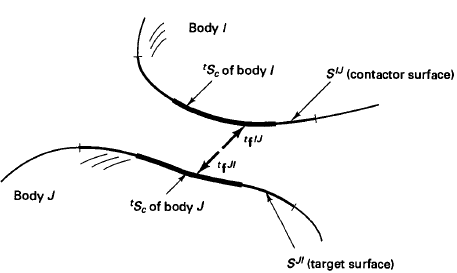
\includegraphics[scale=0.9]{src/ch2/body_contacts.png}
\captionof{figure}{Esquema del contacto entre dos cuerpos}
\label{fig:body_contacts}
\end{center}

En la figura \ref{fig:body_contacts} muestra un esquema para el caso de dos cuerpos, 
denotados como $I$ y $J$ respectivamente. Se asume que cada cuerpo está sujeto de
modo que si no hay contacto no exista un movimiento de cuerpo rígido. Sea $^tF^{IJ}$ 
el vector de las fuerzas de la superficie de contacto en el cuerpo $I$ debido 
al contacto con el cuerpo $J$, entonces $^tf^{IJ} = -^tf^{JI}$. Por lo tanto, 
el trabajo virtual debido a las fuerzas de contacto en \ref{eq:contact_n} puede 
ser escrito como:

\begin{equation}
\int_{S^{IJ}} \delta u_i^I ^tf_i^{IJ} \, dS^{IJ} + 
\int_{S^{JI}} \delta u_i^J ^tf_i^{JI} \, dS^{JI} = 
\int_{S^{IJ}} \delta u_i^{IJ} ^tf_i^{IJ} \, dS^{IJ}
\end{equation}

Donde $\delta u_i^I$ y $\delta u_i^J$ son las componentes del desplazamiento virtual en 
las superficies de contacto de los cuerpos $I$ y $J$, respectivamente, y:

\begin{equation}
\delta u_i^{IJ} = \delta u_i^I - \delta u_i^J
\end{equation}

Comúnmente se llama \textit{pares de contacto} a las superficies $S^{IJ}$ y $S^{JI}$, mismas 
que no necesariamente son del mismo tamaño. Es conveniente llamar a $S^{IJ}$ la 
\textit{superficie contactora} y a $S^{JI}$ la \textit{superficie objetivo}.\\

Tomando como referencia la figura \ref{fig:contact_analysis}, sea $\vec{n}$ el vector unitario 
normal a $S^{JI}$ y sea $\vec{s}$ un vector unitario de tal manera que $\vec{n}$ y $\vec{s}$ formen un base 
ortonormal derecha. Se puede descomponer la fuerza de contacto $^tf^{IJ}$ actuando en $S^{IJ}$ en 
sus componentes normal y tangencial correspondientes a $\vec{n}$ y $\vec{s}$ en $S^{JI}$,

\begin{equation} \label{eq:contact_01}
^tf^{IJ} = \lambda \vec{n} + t \vec{s}
\end{equation}

Donde $\lambda$ y $t$ son las componentes normal y tangencial de la fuerza. Por consiguiente:

\begin{equation}
\lambda = \left( ^tf^{IJ} \right)^T \vec{n}; \,\,\,\,\,\,\,\,\,\, t = \left( ^tf^{IJ} \right)^T \vec{S}
\end{equation}

\begin{center}
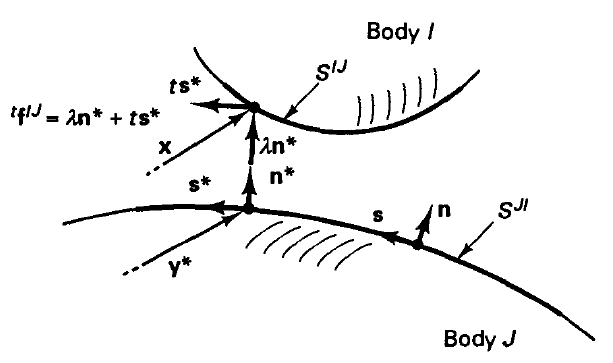
\includegraphics[scale=0.65]{src/ch2/contact_analysis.png}
\captionof{figure}{Esquema del análisis de contactos}
\label{fig:contact_analysis}
\end{center}

Para definir el valor actual de $\vec{n}$,  $\vec{s}$ que se utiliza en los cálculos de contacto, 
considere un punto genérico $\vec{x}$ en $S^{IJ}$ y sea $\vec{y^{\ast}}(\vec{x}, t)$ el punto en $S^{JI}$ 
que satisface: ~\cite{bathe1996}

\begin{equation}
\left\Vert \vec{x} - \vec{y^{\ast}}(\vec{x}, t) \right\Vert_2 = \min \left\{ \Vert \vec{x} - \vec{y} \Vert_2 \right\}
\end{equation}

La distancia de $\vec{x}$ a $S^{JI}$ está dada por:

\begin{equation}
g(\vec{x}, t) = (\vec{x} - \vec{y^{\ast}})^T \vec{n^{\ast}}
\end{equation}

Donde $\vec{n^{\ast}}$ es el vector normal unitario que se utilizó en $\vec{y^{\ast}}(\vec{x}, t)$ y 
$\vec{n^{\ast}}, \, \vec{s^{\ast}}$ son usadas en \ref{eq:contact_01} correspondiendo al punto 
$\vec{x}$. La función $g$ es la función de espaciamiento (\textit{gap function}) para el par 
de la superficie de contacto.\\

Con estas definiciones, las condiciones para el contacto normal puede ser escrito como:

\begin{equation}
g \ge 0;\,\,\,\,\,\, \lambda \ge 0; \,\,\,\,\,\,  g\lambda = 0
\end{equation}

Donde la última ecuación expresa el hecho que si $g > 0$, entonces se tendrá  $\lambda = 0$, 
y viceversa.\\

Para incluir las condiciones de fricción, se asume que la ley de Coulomb se cumple en cada 
nodo de la superficie de contacto y que $\mu$ es el coeficiente de fricción. Esta suposición 
significa por supuesto que los efectos friccionales son incluidos de una forma simplificada.
Primero, se define una variable adimensional $\tau$ dada por:

\begin{equation}
\tau = \frac{t}{\mu \lambda}
\end{equation}

donde $\mu \lambda$ es la resistencia friccional, y la magnitud de la velocidad tangencial relativa 
viene expresada por:

\begin{equation}
\dot{u} (\vec{x}, t) = \left( \vec{\dot{u}} ^J|_{\vec{y^{\ast}}(\vec{x},t)}  - 
\vec{\dot{u}} ^I|_{(\vec{x},t)} | \right) \cdot \vec{s^{\ast}}
\end{equation}

Correspondiente a la vector tangencial unitario $\vec{s}$ en $\vec{y^{\ast}}(\vec{x},t)$. 
Por lo tanto, $ \dot{u}(\vec{x}, t) \vec{s^{\ast}}$ es la velocidad tangencial en el tiempo 
$t$ del punto material en $\vec{y^{\ast}}$ relativo al punto material en $\vec{x}$. Con 
estas definiciones de la ley de Coulomb se tienen las siguientes condiciones:

\begin{equation}
\left\{}
\begin{matrix}
|\tau| \le 1 \\
|\tau| < 1 \,\,\, \text{implica que} \,\,\, \dot{u} = 0 \\
|\tau| = 1 \,\,\, \text{implica que} \,\,\, sign(\dot{u}) = sign(\tau)
\end{matrix}
\right.
\end{equation}


\subsection{Integración implícita vs explícita}

Existen, de manera general, dos tipos de métodos para resolver ecuaciones diferenciales  
en problemas dependientes del tiempo: integración implícita e integración explícita. El 
método implícito de integración en el tiempo puede ser expresado como: ~\cite{nielsen1997}

\begin{equation}
u_{n+1}=f(\dot{u}_{n+1},\ddot{u}_{n+1},u_n,\dot{u}_n,…)
\end{equation}

y el método explícito como:

\begin{equation}
u_{n+1}=f(u_n,\dot{u}_n,\ddot{u}_n,u_{n-1},\dot{u}_{n-1},…)
\end{equation}

El método implícito requiere conocer las derivadas temporales en el paso n+1, las cuales son desconocidas, 
mientras el método explícito está basado en los valores conocidos en el paso n. Si el problema es no 
lineal, el método implícito necesita un procedimiento iterativo para determinar los nuevos desplazamientos. 
Con el método explícito los nuevos desplazamientos se determinan directamente de los valores conocidos 
en pasos previos, evitando el uso de iteraciones adicionales.~\cite{nielsen1997}\\

La simulación de estampados se caracteriza por las diversas no linealidades presentes, debidas al 
material, y a los contactos entre los diversos cuerpos analizados. Sin embargo, usando la integración 
explícita estas no linealidades pueden ser tratadas sin mayores problemas. Por ello, en la mayoría de 
las simulaciones de estampados suelen ser conveniente el uso de algoritmos de integración explícita.


\subsection{Implementación del método en problemas de ingeniería}

\begin{center}
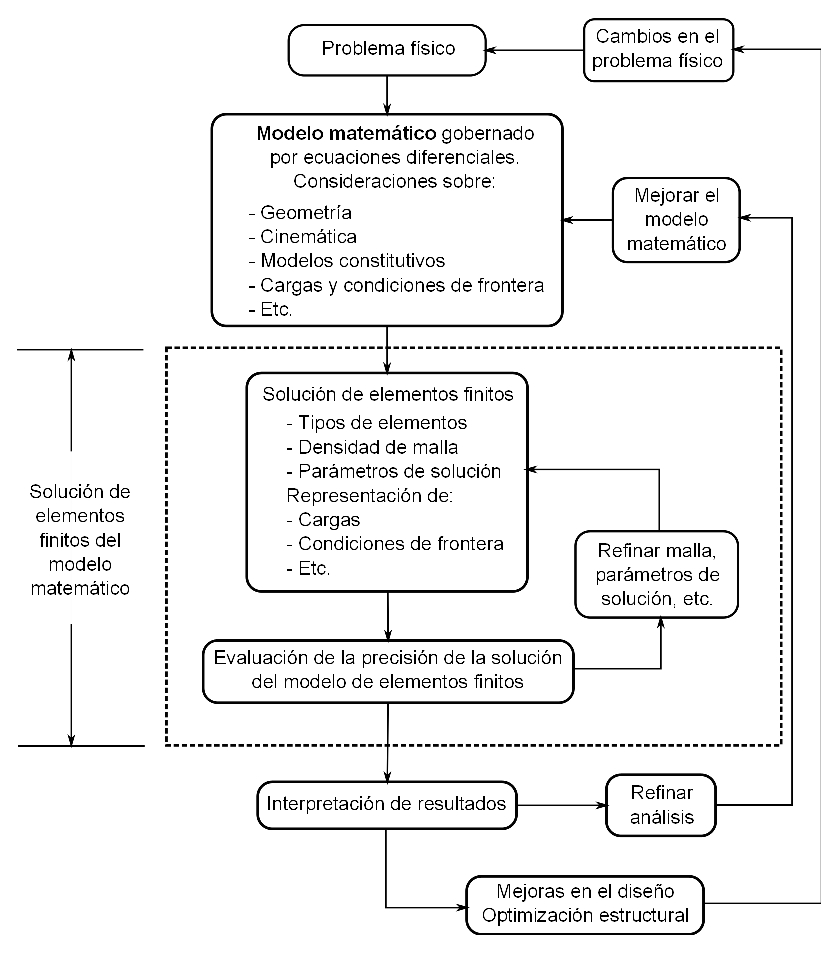
\includegraphics[scale=0.85]{src/ch2/elemento_finito_diagrama}
\captionof{figure}{Diagrama de la implementación del FEM en la solución de problemas de ingeniería}
\label{fig:fem_diagram}
\end{center}


\section{Extensometría} 

La extensometría es la técnica más utilizada para el análisis experimental de tensiones. Su
fundamento básico es la variación de la resistencia producida en un hilo de conductor cuando se alarga
o contrae, y se emplea también en otras aplicaciones como por ejemplo la construcción de
transductores.

\subsection{Teoría básica}

La expresión \ref{eq:res_elect} proporciona la resistencia eléctrica de un conductor 
cilíndrico de diámetro $D$, logitud $l$ y resistividad $\rho$:

\begin{equation}\label{eq:res_elect}
R = \rho \frac{4l}{\pi D^2}
\end{equation}

Derivando la expresión anterior y suponiendo que $\rho$ es independiente de la deformación:

\begin{equation}\label{eq:xxx01}
dR = 4\rho \frac{dl\,\pi D^2 - l\,2\pi D \, dD}{\pi^2 D^4} = 
4\rho \frac{dl}{\pi D^2} - 4\rho \frac{2l\,dD}{\pi D^3}
\end{equation}

A partir de la ecuación anterior se puede hallar la variación de resistencia relativa:

\begin{equation}\label{eq:xxx02}
\frac{dR}{R} = \frac{dl}{l} - 2 \frac{dD}{D}
\end{equation}

Teniendo en cuenta la relación entre deformaciones longitudinales y transversales (efecto Poisson) 
la ecuación \ref{eq:xxx02} puede simplificarse utilizando el módulo de Poisson, $\nu$:

\begin{equation}
\frac{dD}{D} = -\nu \frac{dl}{l} \\ 
\frac{dR}{R} = (1 + 2\nu) \frac{dl}{l} = K \cdot \epsilon
\end{equation}






